
\newcommand{\insimg}[1] {
  \begin{subfigure}[b]{0.2\textwidth}
    \centering
    \includegraphics[keepaspectratio=true, width=\textwidth]{images/#1}
  \end{subfigure}
}

\chapter{性能测试}
\label{chap:benchmark}

为了测试本系统的可用性,需要测试检索算法的鲁棒性和效率。

\section{测试指标}
\label{sec:benchmark-index}
鲁棒性:本系统利用DCT抽取出图像的特征向量,采用向量间的距离作为图片的
相似程度的度量,距离越大,图片相似程度越低,同理,距离越小(大于0),
图片的相似程度就越高。对鲁棒性的测试应着眼于在不同情况下,加噪图与
原图的距离的变化情况,距离越小,抗噪声性能越好。

效率:本系统接受一个待检索图后,在特征数据库中检索所有的特征向量后返回
前10相似的图片。对效率的测试应着眼于系统检索出结果的时间,以及客户端接
收到全部结果图片的时间,检索时间越小,服务端检索性能越好,接受时间越
小,客户端性能越好。

\section{测试方案}
\label{sec:benchmark-scheme}

\begin{itemize}
\item 为了测试检索算法的鲁棒性,拟选择一些样本图片,并对这些样本做一些典型的
变化:
\begin{itemize}
\item 加入椒盐噪声
\item 改变质量因子$Q$
\end{itemize}
然后统计加噪图与原图的距离。

\item 为了测试检索算法的效率,拟在同一台主机上同时开启本系统的服务端和客户端,
即在忽略网络状况的情况下测试系统的检索速度并统计时间。
\end{itemize}

\section{测试环境}
\label{sec:benchmark-env}

\begin{itemize}
\item 硬件环境:
\begin{itemize}
\item 处理器:Intel Core i5-2410M CPU @ 2.30GHz
\item 内存:4.00GB(3.82GB可用)
\end{itemize}
\item 软件环境:
\begin{itemize}
\item 操作系统:Windows 8 专业版 x64(含Media Center) 
\item Python 2.7.3 x86
\item numpy 1.7.1
\item opencv-python-2.4.5
\end{itemize}
\end{itemize}

\section{测试数据}
\label{sec:benchmark-data}

测试图像集为37张灰度人脸图,大小为$640 \times 480$,单位为像素。
图集如下图

\begin{figure}[H]
  \centering
  \insimg{gs0.jpg}
  \insimg{gs1.jpg}
  \insimg{gs2.jpg}
  \insimg{gs3.jpg}
  \vspace{0.1cm}

  \insimg{gs4.jpg}
  \insimg{gs5.jpg}
  \insimg{gs6.jpg}
  \insimg{gs7.jpg}
  \vspace{0.1cm}

  \insimg{gs8.jpg}
  \insimg{gs9.jpg}
  \insimg{gs10.jpg}
  \insimg{gs11.jpg}
  \vspace{0.1cm}

  \insimg{gs12.jpg}
  \insimg{gs13.jpg}
  \insimg{gs14.jpg}
  \insimg{gs15.jpg}
  \vspace{0.1cm}

  \insimg{gs16.jpg}
  \insimg{gs17.jpg}
  \insimg{gs18.jpg}
  \insimg{gs19.jpg}
  \vspace{0.1cm}
\end{figure}
\begin{figure}[H]
  \centering

  \insimg{gs20.jpg}
  \insimg{gs21.jpg}
  \insimg{gs22.jpg}
  \insimg{gs23.jpg}
  \vspace{0.1cm}

  \insimg{gs24.jpg}
  \insimg{gs25.jpg}
  \insimg{gs26.jpg}
  \insimg{gs27.jpg}
  \vspace{0.1cm}

  \insimg{gs28.jpg}
  \insimg{gs29.jpg}
  \insimg{gs30.jpg}
  \insimg{gs31.jpg}
  \vspace{0.1cm}

  \insimg{gs32.jpg}
  \insimg{gs33.jpg}
  \insimg{gs34.jpg}
  \insimg{gs35.jpg}
  \vspace{0.1cm}

  \insimg{gs36.jpg}
\end{figure}


\section{测试结果及分析}
\label{sec:result-and-analysis}

\subsection{椒盐噪声}
\label{sec:speckle-data}

典型的加入椒盐噪声的图如下
\begin{figure}[H]
  \centering
  \begin{subfigure}[b]{0.4\textwidth}
    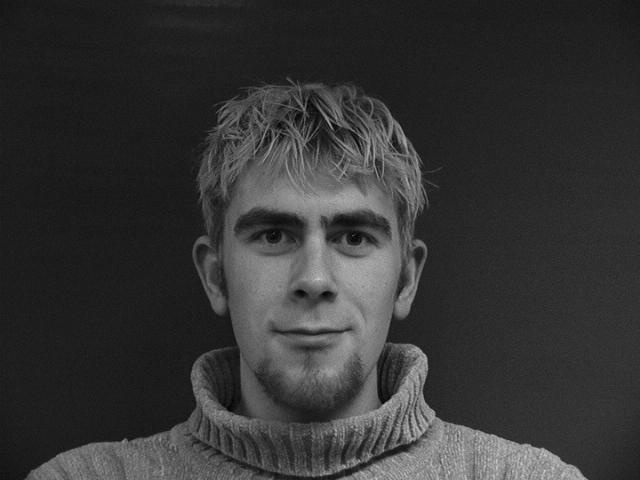
\includegraphics[keepaspectratio=true,
    width=\textwidth]{images/gs0.jpg}
    \caption{原图}
  \end{subfigure}
  \begin{subfigure}[b]{0.4\textwidth}
    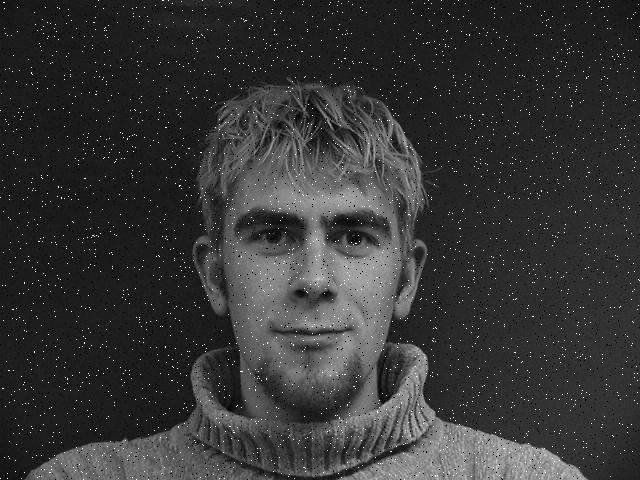
\includegraphics[keepaspectratio=true,
    width=\textwidth]{images/gs0_0.02_speckle.jpg}
    \caption{加噪图}
  \end{subfigure}
  \caption{噪声参数为0.02时的椒盐噪声对gs0.jpg的影响}
\label{fig:speckle-ex-img}
\end{figure}

对上示原图加入噪声密度在$[0, 0.1]$内、步长为0.01的椒盐噪声后,分别统计
与原图的距离,可作如下的散点图
\begin{figure}[H]
  \centering
  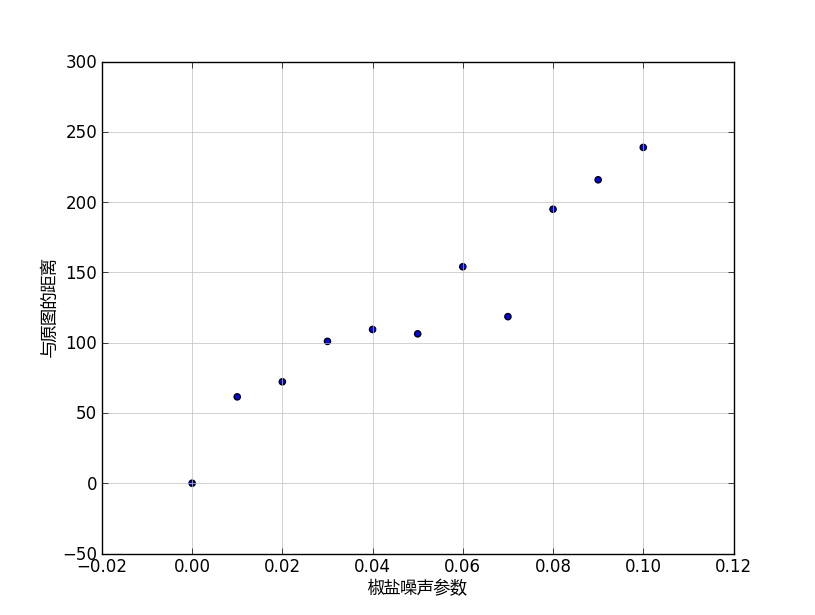
\includegraphics[keepaspectratio=true,
  scale=0.6]{images/speckle_gs0.png}
  \caption{对gs0.jpg的椒盐噪声统计}
  \label{fig:speckle-gs0-scatter-plot}
\end{figure}

为不失一般性,选取37张图片做同样处理,统计出散点图,如图
\begin{figure}[H]
  \centering
  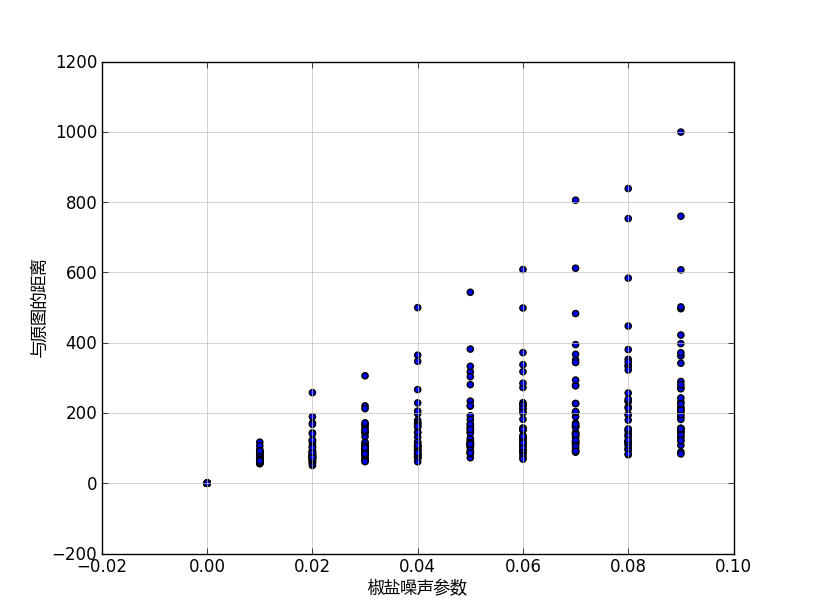
\includegraphics[keepaspectratio=true,
  scale=0.6]{images/speckle_all.png}
  \caption{对所有图片的椒盐噪声统计}
  \label{fig:speckle-all-scatter-plot}
\end{figure}

从图中可以看出来,本算法可以抵抗噪声密度小于$0.1$的椒盐噪声,在此噪声
密度下,加噪图与原图距离普遍小于$500$,当噪声密度大于$0.1$后,加噪图
与原图距离增大到了无法接受的地步。

\subsection{质量因子}
\label{sec:quality-data}

原图与质量因子$Q = 10$时的图如下
\begin{figure}[H]
  \centering
  \begin{subfigure}[b]{0.4\textwidth}
    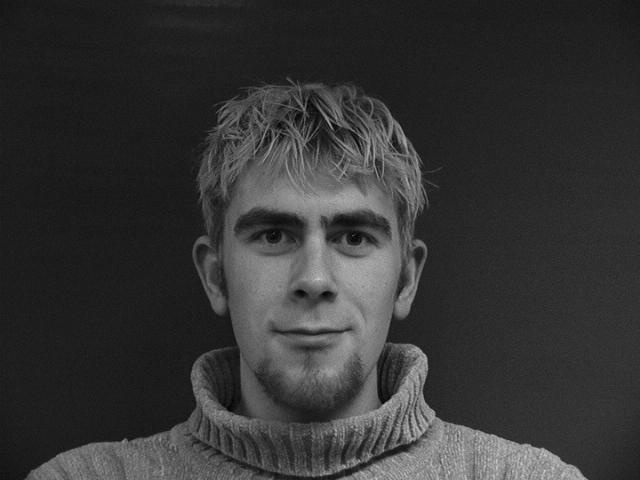
\includegraphics[keepaspectratio=true,
    width=\textwidth]{images/gs0.jpg}
    \caption{原图}
  \end{subfigure}
  \begin{subfigure}[b]{0.4\textwidth}
    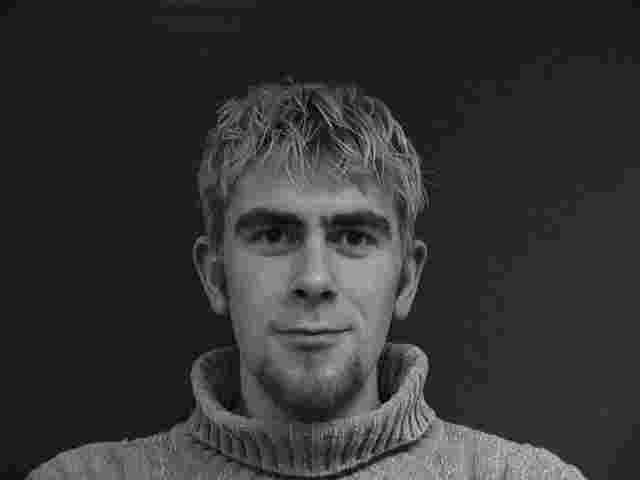
\includegraphics[keepaspectratio=true,
    width=\textwidth]{images/gs0_0.10_quality.jpg}
    \caption{压缩图}
  \end{subfigure}
  \caption{质量因子为10时的压缩操作对gs0.jpg的影响}
\label{fig:quality-ex-img}
\end{figure}

调整上示原图的质量因子$Q \in [0, 1]$、步长为$0.1$(在$[0.9, 1]$之间步长
为$0.01$)后,分别统计与原图的距离,可作如下的散点图
\begin{figure}[H]
  \centering
  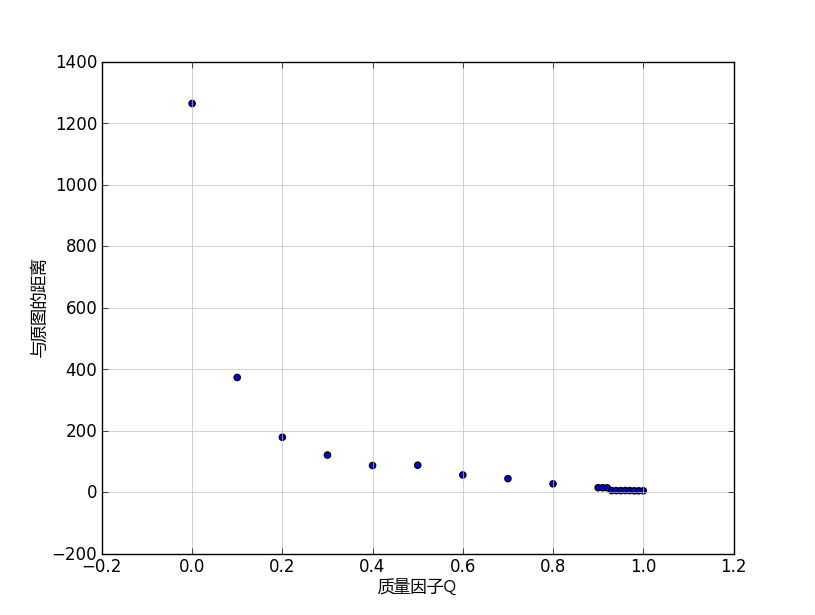
\includegraphics[keepaspectratio=true,
  scale=0.6]{images/quality_gs0.png}
  \caption{对gs0.jpg的压缩操作统计}
  \label{fig:quality-gs0-scatter-plot}
\end{figure}

\begin{figure}[H]
  \centering
  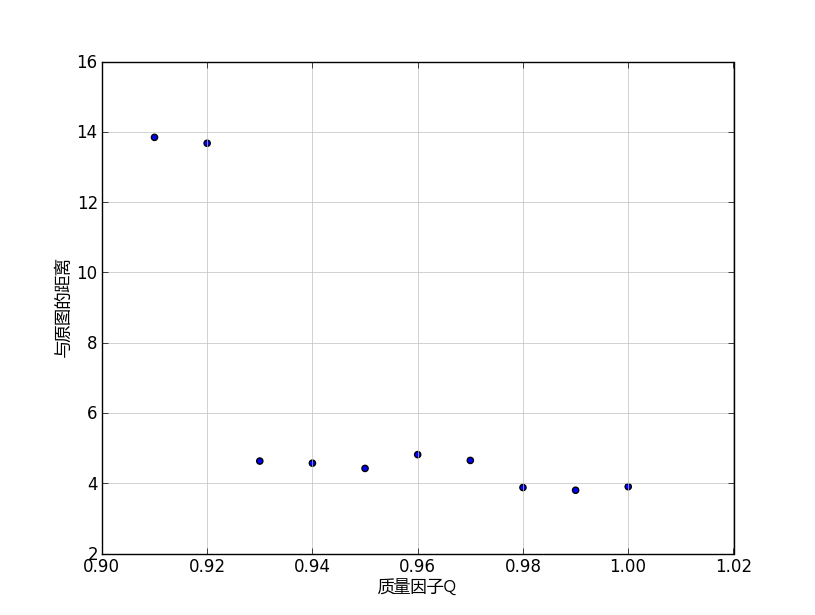
\includegraphics[keepaspectratio=true,
  scale=0.6]{images/quality_gs0_0.9_1.png}
  \caption{对gs0.jpg的压缩操作统计($[0.9, 1]$区间)}
  \label{fig:quality-gs0-sub-scatter-plot}
\end{figure}

为不失一般性,选取37张图片做同样处理,统计出散点图,如图
\begin{figure}[H]
  \centering
  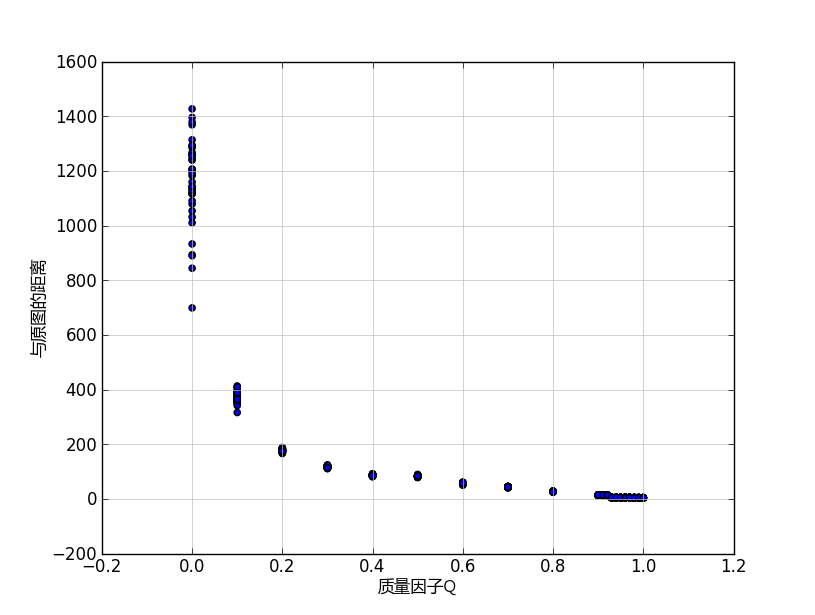
\includegraphics[keepaspectratio=true,
  scale=0.6]{images/quality_all.png}
  \caption{对所有图片的压缩操作统计}
  \label{fig:quality-all-scatter-plot}
\end{figure}

\begin{figure}[H]
  \centering
  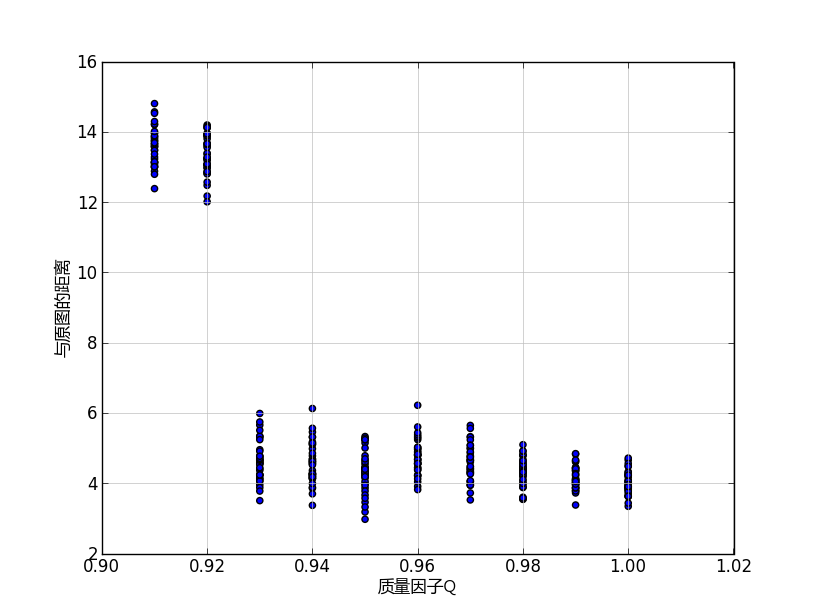
\includegraphics[keepaspectratio=true,
  scale=0.6]{images/quality_all_0.9_1.png}
  \caption{对所有图片的压缩操作统计($[0.9, 1]$区间)}
  \label{fig:quality-gs0-sub-scatter-plot}
\end{figure}

从图中可以看出来,本算法有较好的抗压缩性能,即使图片质量被调整为$10\%$,
与原图的距离仍然小于$500$。

\subsection{系统检索效率}
\label{sec:sys-retrieval-effi}

使用gs0.jpg做10次检索,分别记录:
\begin{itemize}
\item 检索耗时$t_r$:服务器比对所有特征向量,获得结果集所花时间;
\item 检索结束耗时$t_a$:客户端从点击\texttt{Retrieve}按钮开始到所有结
  果图像获取结束所花时间。
\end{itemize}

测试结果如下表


\begin{table}[H]
  \setlength{\tabcolsep}{25pt}
  \centering
  \begin{tabular}{ l c c }
    \hline
    序号 & $t_r$ & $t_a$ \\ \hline \hline
    1 & $0.08562$ & $3.44197$ \\
    2 & $0.08107$ & $3.50858$ \\
    3 & $0.08263$ & $3.42089$ \\
    4 & $0.08283$ & $3.46747$ \\
    5 & $0.08285$ & $3.50209$ \\
    6 & $0.11238$ & $3.50387$ \\
    7 & $0.08241$ & $3.43419$ \\
    8 & $0.08106$ & $3.50417$ \\
    9 & $0.08139$ & $3.44271$ \\
    10 & $0.08165$ & $3.46871$ \\
    均值 & $0.08539$ & $3.46947$ \\
    \hline
  \end{tabular}
  \caption{系统效率测试结果}
  \label{tab:sys-retrieval-effi}
\end{table}



该表显示出本系统的检索耗时$t_r$较小,即服务端检索性能较好,但检索结束
耗时$t_a$高出$t_r$很多,原因可能是base64加解码与图像加解密比较耗时。
